\section{Prostory s~mírou}\label{sec:prostory-s-mirou}

Jak již bylo zmíněno v~úvodu,~klíčovým pojmem v~této kapitole (a pro studium fraktálů obecně) je takzvaná \emph{míra}. Ta pro nás představuje obecný způsob,~jak můžeme množinám přiřadit v~jistém smyslu "velikost". Konkrétněji,~byť vágně,~lze říci,~že sestává-li množina z konečného nebo spočetného množství "rozumných" částí,~pak součet velikostí všech těchto dílčích množin je roven velikosti celé množiny,~kterou nazveme její \emph{mírou}. Pro začátek celkem jednoduchá myšlenka.

Pro formální zavedení tohoto pojmu však budeme muset nejprve zavést ještě jiný pojem,~a to tzv. \emph{$\sigma$-algebru}.

\subsection{Měřitelné prostory}\label{subsec:meritelne-prostory}

\begin{definition}[$\sigma$-algebra]\label{def:sigma-algebra}
    Nechť je dána libovolná množina $X$ a systém podmnožin $\mathcal{A}\subseteq\powset{X}$. Pak $\mathcal{A}$ je \emph{$\sigma$-algebra}\index{měřitelný prostor!$\sigma$-algebra} na množině $X$,~pokud:
    \begin{enumerate}[label=(\alph*)]
        \item\label{def:sigma-algebra-podm1} $X\in\mathcal{A}$.
        \item\label{def:sigma-algebra-podm2} Pro každou množinu $A\in\mathcal{A}$ platí $X\setminus A\in\mathcal{A}$.
        \item\label{def:sigma-algebra-podm3} Pro libovolné množiny $A_1,A_2,\ldots\in\mathcal{A}$ platí $\bigcup_{i=1}^\infty A_i\in\mathcal{A}$.
    \end{enumerate}
    Dvojice $(X,\mathcal{A})$ se nazývá měřitelný prostor\index{měřitelný prostor}.
\end{definition}
\todo{Psát na konci každého bodu v~definici/větě \textbf{tečku},~\textbf{čárku} nebo \textbf{středník}?}

\begin{example}
    Jednoduché příklady $\sigma$-algeber:
    \begin{itemize}
        \item Triviálními příklady $\sigma$-algeber jsou množiny $\emptyset$,~$\powset{X}$ a~$\set{\emptyset,X}$ pro libovolnou množinu $X$.
        \item Pro konečnou množinu $X=\set{a,b,c,d}$ je jednou možnou $\sigma$-algebrou systém množin
        \[\Sigma=\set{\emptyset,\set{a,b},\set{c,d},\set{a,b,c,d}}.\]
    \end{itemize}
    Sami se zkuste přesvědčit,~že všechny zmíněné příklady vyhovují definici \ref{def:sigma-algebra}.
\end{example}

Než vyslovíme něco dalšího o~$\sigma$-algebrách a jejich významu,~podíváme se na seznam některých vesměs jednoduchých pozorováních zformulovaných níže v~tvrzení \ref{thm:sigma-algebra-vlastnosti}.
\begin{theorem}[Vlastnosti $\sigma$-algebry]\label{thm:sigma-algebra-vlastnosti}
    Nechť $(X,\mathcal{A})$ je meřitelný prostor. Pak platí:
    \begin{enumerate}[label=(\roman*)]
        \item $\emptyset\in\mathcal{A}$.
        \item Pro libovolné množiny $A_1,A_2,\ldots\in\mathcal{A}$ platí $\bigcap_{i=1}^\infty A_i\in\mathcal{A}$.
        \item Pro všechny množiny $A_1,A_2,\ldots,A_n\in\mathcal{A}$ platí
        \[\bigcup_{i=1}^n A_i\in\mathcal{A}\land\bigcap_{i=1}^n A_i\in\mathcal{A}.\]
        \item Jsou-li $A,B\in\mathcal{A}$ pak $A\setminus B\in\mathcal{A}$.
    \end{enumerate}
\end{theorem}

Z tohoto tvrzení je již lépe vidět,~proč jsou pro nás $\sigma$-algebry tak příjemným objektem. Jsou totiž \emph{uzavřené} na všechny základní množinové operace. To se nám bude později hodit při zavedení míry,~ke které směřujeme. Důkaz těchto dílčích tvrzení přitom není nikterak složitý.
\begin{proof}
    Mějme $\sigma$-algebru $\mathcal{A}$ na množině $X$.
    \begin{enumerate}[label=\textit{(\roman*)}]
        \item Z podmínky \ref{def:sigma-algebra-podm1} definice \ref{def:sigma-algebra} víme,~že $X\in\mathcal{A}$ a z podmínky \ref{def:sigma-algebra-podm2} tedy plyne $X\setminus X=\emptyset\in\mathcal{A}$.
        \item Mějme množiny $A_1,A_2,\ldots\in\mathcal{A}$. Společně s~využitím De Morganových zákonů plyne následující:
        \[\bigcap\limits_{i=1}^\infty A_i=\overbrace{X\setminus\underbrace{\bigcup\limits_{i=1}^\infty \overbrace{(X\setminus A_i)}^{\text{$\in\mathcal{A}$ podle \ref{def:sigma-algebra-podm2}}}}_{\text{$\in\mathcal{A}$ podle \ref{def:sigma-algebra-podm3}}}}^\text{$\in\mathcal{A}$ podle \ref{def:sigma-algebra-podm2}}\in\mathcal{A}.\]
        \item Nechť jsou dány množiny $A_1,A_2,\ldots,A_n\in\mathcal{A}$. Když pro každé $j>n$ položíme $A_j=\emptyset$,~pak platí
        \[\bigcup\limits_{i=1}^n A_i=\bigcup\limits_{i=1}^\infty A_i\in\mathcal{A}\]
        a podobně pro $\bigcap_{i=1}^n A_i\in\mathcal{A}$ podle předešlého bodu.
        \item Pro libovolné množiny $A,B\in\mathcal{A}$ platí
        \[A\setminus B=\overbrace{A\cup\underbrace{(X\setminus B)}_{\text{$\in\mathcal{A}$ podle \ref{def:sigma-algebra-podm2}}}}^{\text{$\in\mathcal{A}$ podle \ref{def:sigma-algebra-podm3}}}\in\mathcal{A}.\]
    \end{enumerate}
\end{proof}

\subsection{Míra}\label{subsec:mira}

V tuto chvíli máme již vše potřebné k~zavedení pojmu míra,~resp. prostor s~mírou.
\begin{definition}[Prostor s~mírou]\label{def:prostor-s-mirou}
    Nechť $(X,\mathcal{A})$ je meřitelný prostor. Zobrazení $\mapping{\mu}{\mathcal{A}}{\langle0,\infty\rangle}$ se nazývá \emph{míra}\index{prostor s~mírou!míra} na $\mathcal{A}$,~pokud platí:
    \begin{enumerate}[label=(\roman*)]
        \item\label{def:mira-podm1} $\mu(\emptyset)=0$,
        \item\label{def:mira-podm2} pro množiny $A_1,A_2,\ldots\in\mathcal{A}$ po dvou disjunktní je
        \[\mu\left(\bigcup\limits_{i=1}^\infty A_i\right)=\sum_{i=1}^\infty\mu(A_i).\mathrightnote{$\sigma$-aditivita}\]
    \end{enumerate}
    Uspořádanou trojici $(X,\mathcal{A},\mu)$ nazýváme \emph{prostor s~mírou}\index{prostor s~mírou}.
\end{definition}

Vzhledem k~tomu,~co míra reprezentuje (tj. zobecnění délky,~obsahu,~objemu),~jsou tyto požadavky intuitivně dosti smysluplné.

\begin{example}\label{ex:mira}
    Příklady prostorů s~mírou:
    \begin{itemize}
        \item Asi pro nás nejtypičtější způsob,~jak měřit "velikost" množiny,~je podle \emph{počtu prvků}. Pro libovolnou množinu $X$ a potenční množinu $\powset{X}$ lze definovat prostor s~mírou $(X,\powset{X},\mu)$,~kde pro libovolnou množinu $A\in\powset{X}$ položíme $\mu(A)=|A|$. Takto definované míře $\mu$ říkáme \emph{aritmetická míra}\index{prostor s~mírou!aritmetická míra}.
        \item Máme libovolnou množinu $X$ a $\sigma$-algebru $\mathcal{A}$. Zvolme si pevně $x\in X$. Míru libovolné množiny $A\in\mathcal{A}$ lze definovat jako $\delta_x(A)=\chi_A(x)$,~kde $\chi_A$ je charakteristická funkce množiny $A$. Zobrazení $\delta_x$ je tzv. \emph{Diracova míra}.
        \item Zobrazení přiřazující náhodnému jevu pravděpodobnost je též případem míry. Označíme-li si $\Omega=\set{\omega_1,\omega_2,\ldots,\omega_n}$ množinu všech elementárních jevů a $\mathcal{F}\subseteq\powset{\Omega}$,~pak $\mapping{\mathsf{P}}{\mathcal{F}}{\langle0,1\rangle}$ definovaná pro $A\in\mathcal{F}$ jako
        \[\mathsf{P}(A)=\dfrac{|A|}{|\Omega|}\]
        je mírou na $\mathcal{F}$. Speciálně $\mathsf{P}(\Omega)=1$.
    \end{itemize}
\end{example}

Ve všech případech zobrazení $\mu$ v~příkladu \ref{ex:mira} se lze snadno přesvědčit,~že se jedná o~míru,~tedy že splňuje podmínky \ref{def:mira-podm1} a \ref{def:mira-podm2} uvedené v~definici \ref{def:prostor-s-mirou} výše.

Pojďme nyní prozkoumat vlastnosti míry trochu hlouběji.
\begin{theorem}[Vlastnosti míry]\label{thm:mira-vlastnosti}
    Nechť $\mu$ je míra na $\sigma$-algebře $\mathcal{A}$. Pak platí následující:
    \begin{enumerate}[label=(\roman*)]
        \item\label{thm:mira-aditivita} Jsou-li množiny $A_1,A_2,\ldots,A_n\in\mathcal{A}$ po dvou disjunktní,~pak
        \[\mu\left(\bigcup_{i=1}^n A_i\right)=\sum_{i=1}^{n}\mu(A_i).\mathrightnote{aditivita\index{aditivita}}\]
        \item\label{thm:mira-monotonie} Pokud $A,B\in\mathcal{A}$ a $A\subseteq B$,~pak
        \[\mu(A)\leqslant\mu(B).\mathrightnote{monotonie míry\index{monotonie míry}}\]
        Navíc pokud $\mu(A)<\infty$,~pak $\mu(B\setminus A)=\mu(B)-\mu(A)$.
        \item\label{thm:mira-nekl-posl} Pokud $A_1,A_2,\ldots$,~kde $A_i\in\mathcal{A}$ pro každé $i\in\N$,~je neklesající posloupnost množin\footnote{Posloupnost množin, kde $A_i\subseteq A_{i+1}$ pro každé $i\in\N$.},~pak
        \[\lim_{j\to\infty}\mu(A_j)=\mu\left(\bigcup_{j=1}^\infty A_j\right).\]
        \item\label{thm:mira-nerost-posl} Pokud $A_1,A_2,\ldots\in\mathcal{A}$ je nerostoucí posloupnost množin\footnote{$A_i\supseteq  A_{i+1}$ pro každé $i\in\N$.} a~navíc $\mu(A_1)<\infty$,~pak
        \[\lim_{j\to\infty}\mu(A_j)=\mu\left(\bigcap_{j=1}^\infty A_j\right).\]
        \item\label{thm:mira-sigma-subaditivita} Pokud $A_1,A_2,\ldots$,~kde $A_i\in\mathcal{A}$ pro každé $i\in\N$,~pak
        \[\mu\left(\bigcup_{i=1}^\infty A_i\right)\leqslant\sum_{i=1}^{\infty}\mu(A_i).\mathrightnote{$\sigma$-subaditivita}\]
    \end{enumerate}
\end{theorem}

Poslední vlastnost \ref{thm:mira-sigma-subaditivita} je tzv. \emph{$\sigma$-subaditivita}\index{$\sigma$-subaditivita}\footnote{V matematické terminologii se předpona $\sigma$ běžně týká spočetných sjednocení. \citep[str. 2]{Lukes2013}}. Oproti $\sigma$-aditivitě\index{$\sigma$-aditivita} se liší tím,~že u~množin $A_1,A_2,\dots$ se nepožaduje,~aby byly po dvou disjunktní,~tzn. mohou se "překrývat". Je však intuitivně nejspíše jasné,~že součtem měr všech těchto množin určitě nemůžeme získat míru větší než je míra jejich sjednocení (dané "překryvy" započítáváme v~sumě vícekrát). Podobně i~monotonie dává intuitivně smysl,~neboť část větší množiny jistě nemůže mít větší míru než celek. Na formální stránku věci se podíváme nyní.
\begin{proof}
    V~důkazu využijeme některé vlastnosti $\sigma$-algebry z věty \ref{thm:sigma-algebra-vlastnosti}, zejména,~že všechny množiny níže jsou opět prvky $\sigma$-algebry~$\mathcal{A}$.
    \begin{enumerate}[label=\textit{(\roman*)}]
        \item Pokud pro každé $j>n$ položíme $A_j=\emptyset$,~pak z definice míry plyne
        \[\mu\left(\bigcup_{i=1}^n A_i\right)=\mu\left(\bigcup_{i=1}^\infty A_i\right)=\sum_{i=1}^{\infty}\mu(A_i)=\sum_{i=1}^{n}\mu(A_i).\]
        \item Nechť jsou dány $A,B\in\mathcal{A}$,~takové,~že $A\subseteq B$. Pak $B=A\cup(B\setminus A)$,~přičemž $A$ a $B\setminus A$ jsou disjunktní. Tedy podle bodu \ref{def:mira-podm2} lze psát $\mu(B)=\mu(A)+\mu(B\setminus A)\geqslant\mu(A)$,~protože $\mu(B\setminus A)\geqslant 0$.
        \item Mějme neklesající posloupnost množin $A_1,A_2,\ldots$,~kde $A_i\in\mathcal{A}$ pro každé $i\in\N$ (viz obrázek \ref{fig:nekl-posl-mnozin}).
        Definujeme posloupnost\footnote{V podstatě konstruujeme množiny $A_1,A_2,\ldots$ tak,~aby v~následující množině $A_i$ nebyl obsažen prvek,~který se nachází již v~některé z množin $A_1,A_2,\ldots,A_{i-1}$. Podobná myšlenka je využita i při důkazu budů \ref{thm:mira-nerost-posl} a \ref{thm:mira-sigma-subaditivita}.} množin $B_1,B_2,\ldots$ následovně:
        \[B_1=A_1,\;B_2=A_2\setminus A_1,\;B_i=A_i\setminus A_{i-1},\;i\geqslant 2.\]
        Množiny $B_1,B_2,\dots$ jsou po dvou disjunktní a zároveň\\$\bigcup_{i=1}^\infty B_i=\bigcup_{i=1}^\infty A_i$. Libovolnou množinu $A_n$ lze totiž zapsat jako
        \[A_n=\bigcup_{i=1}^n (A_i\setminus A_{i-1})=\bigcup_{i=1}^n B_i.\] 
        Podle již dokázaného bodu \ref{thm:mira-aditivita} (aditivita míry) tedy pro každé $n$ platí $\mu(A_n)=\sum_{i=1}^{n}\mu(B_i)$.
        Celkově
        \[\mu\left(\bigcup_{i=1}^\infty A_i\right)=\mu\left(\bigcup_{i=1}^\infty B_i\right)=\sum_{i=1}^{\infty}\mu(B_i)=\lim_{n\to\infty}\sum_{i=1}^{n}\mu(B_i)=\lim_{n\to\infty}\mu(A_n).\]
        \item Nechť je dána nerostoucí posloupnost množin $A_1,A_2,\ldots$,~kde $A_i\in\mathcal{A}$ pro každé $i\in\N$ (viz obrázek \ref{fig:nerost-posl-mnozin}). Podobně jako v~předešlém bodě,~i~zde definujeme novou posloupnost množin $B_1,B_2,\ldots$ takto:
        \[B_i=A_1\setminus A_i,\;i\in\N.\]
        Zde si můžeme všimnout,~že pro každé $i$ platí $B_i\subseteq B_{i+1}$ a splňuje tak předpoklad předešlého bodu \ref{thm:mira-nekl-posl}. Dle De Morganových zákonů můžeme psát
        \[\bigcup_{i=1}^\infty B_i=\bigcup_{i=1}^\infty(A_1\setminus A_i)=A_1\setminus\bigcap_{i=1}^\infty A_i.\]
        Výraz $\lim_{j\to\infty}B_j$ lze rozepsat dvěma způsoby:
        \begin{align*}
            \lim\limits_{j\to\infty}\mu(B_j)&\stackrel{\ref{thm:mira-nekl-posl}}{=}\mu\left(\bigcup\limits_{i=1}^\infty B_i\right)=\mu\left(A_1\setminus\bigcap\limits_{i=1}^\infty A_i\right)\stackrel{\ref{thm:mira-monotonie}}{=}\mu(A_1)-\mu\left(\bigcap\limits_{i=1}^\infty A_i\right),\\
            \lim\limits_{j\to\infty}\mu(B_j)&=\lim_{j\to\infty}(A_1\setminus A_j)\stackrel{\ref{thm:mira-monotonie}}{=}\lim_{j\to\infty}(\mu(A_1)-\mu(A_j))=\mu(A_1)-\lim_{j\to\infty}\mu(A_j).
        \end{align*}
        Porovnáním obou rovností lze vidět,~že
        \[\lim_{j\to\infty}\mu(A_j)=\mu\left(\bigcap\limits_{i=1}^\infty A_i\right).\]
        \item Nechť jsou dány množiny $A_1,A_2,\ldots$, kde $A_i\in\mathcal{A}$ pro každé $i\in\N$. Definujeme posloupnost množin $B_1,B_2,\ldots$ takto:
        \[B_1=A_1,\;B_i=A_i\setminus\bigcup_{i=1}^{k-1} A_i.\]
        Není složité si rozmyslet,~že množiny $B_1,B_2,\ldots$ jsou po dvou disjunktní. Zároveň platí $\bigcup_{i=1}^\infty B_i=\bigcup_{i=1}^\infty A_i$ a $B_j\subseteq A_j$ pro každé $j\in\N$. Tím je dokázáno,~že
        \[\mu\left(\bigcup_{i=1}^\infty A_i\right)=\mu\left(\bigcup_{i=1}^\infty B_i\right)=\sum_{i=1}^{\infty}\mu(B_i)\stackrel{\ref{thm:mira-monotonie}}{\leqslant}\sum_{i=1}^{\infty}\mu(A_i).\]
    \end{enumerate}
    \begin{figure}[h]
        \centering
        \begin{subfigure}{0.45\textwidth}
            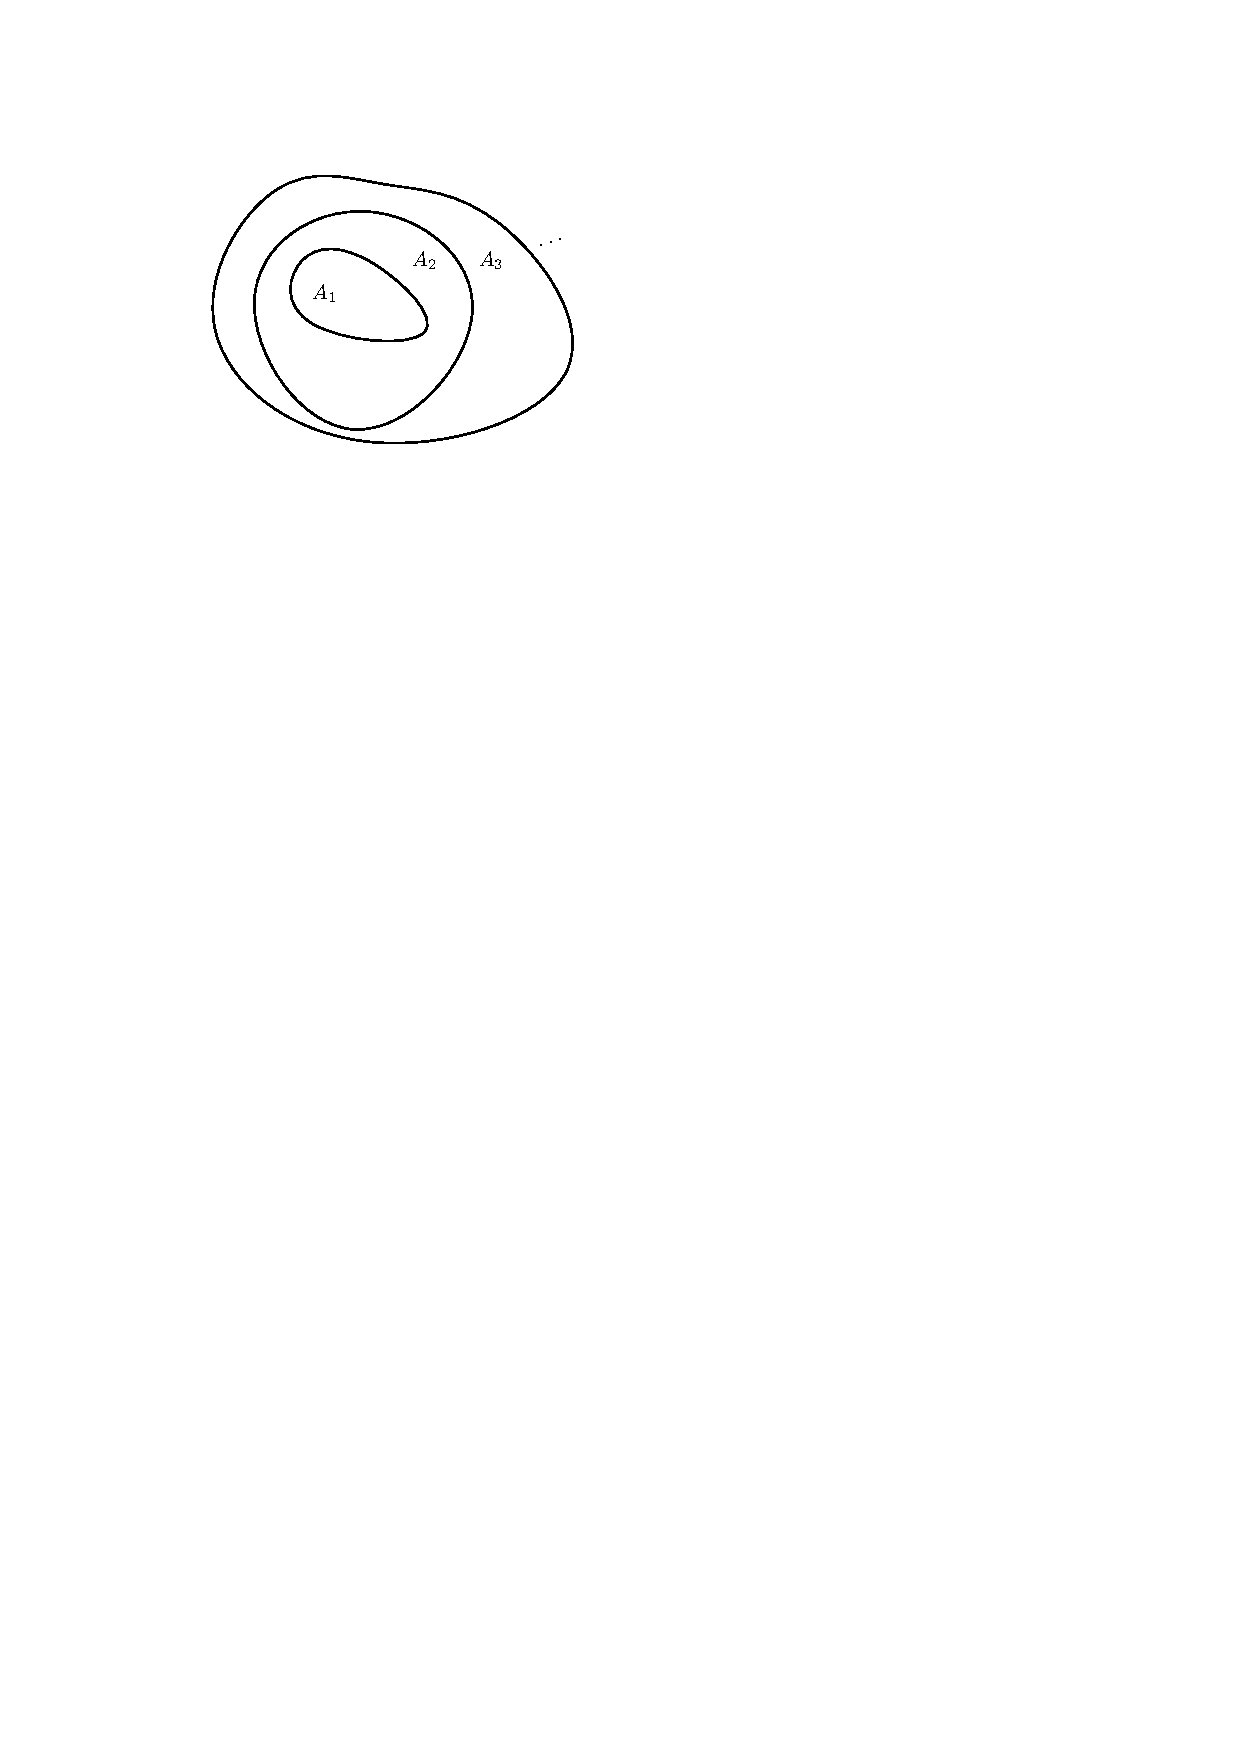
\includegraphics{ch02-neklesajici-posl-mnozin.pdf}
            \caption{Neklesající posloupnost množin}
            \label{fig:nekl-posl-mnozin}
        \end{subfigure}
        \qquad
        \begin{subfigure}{0.45\textwidth}
            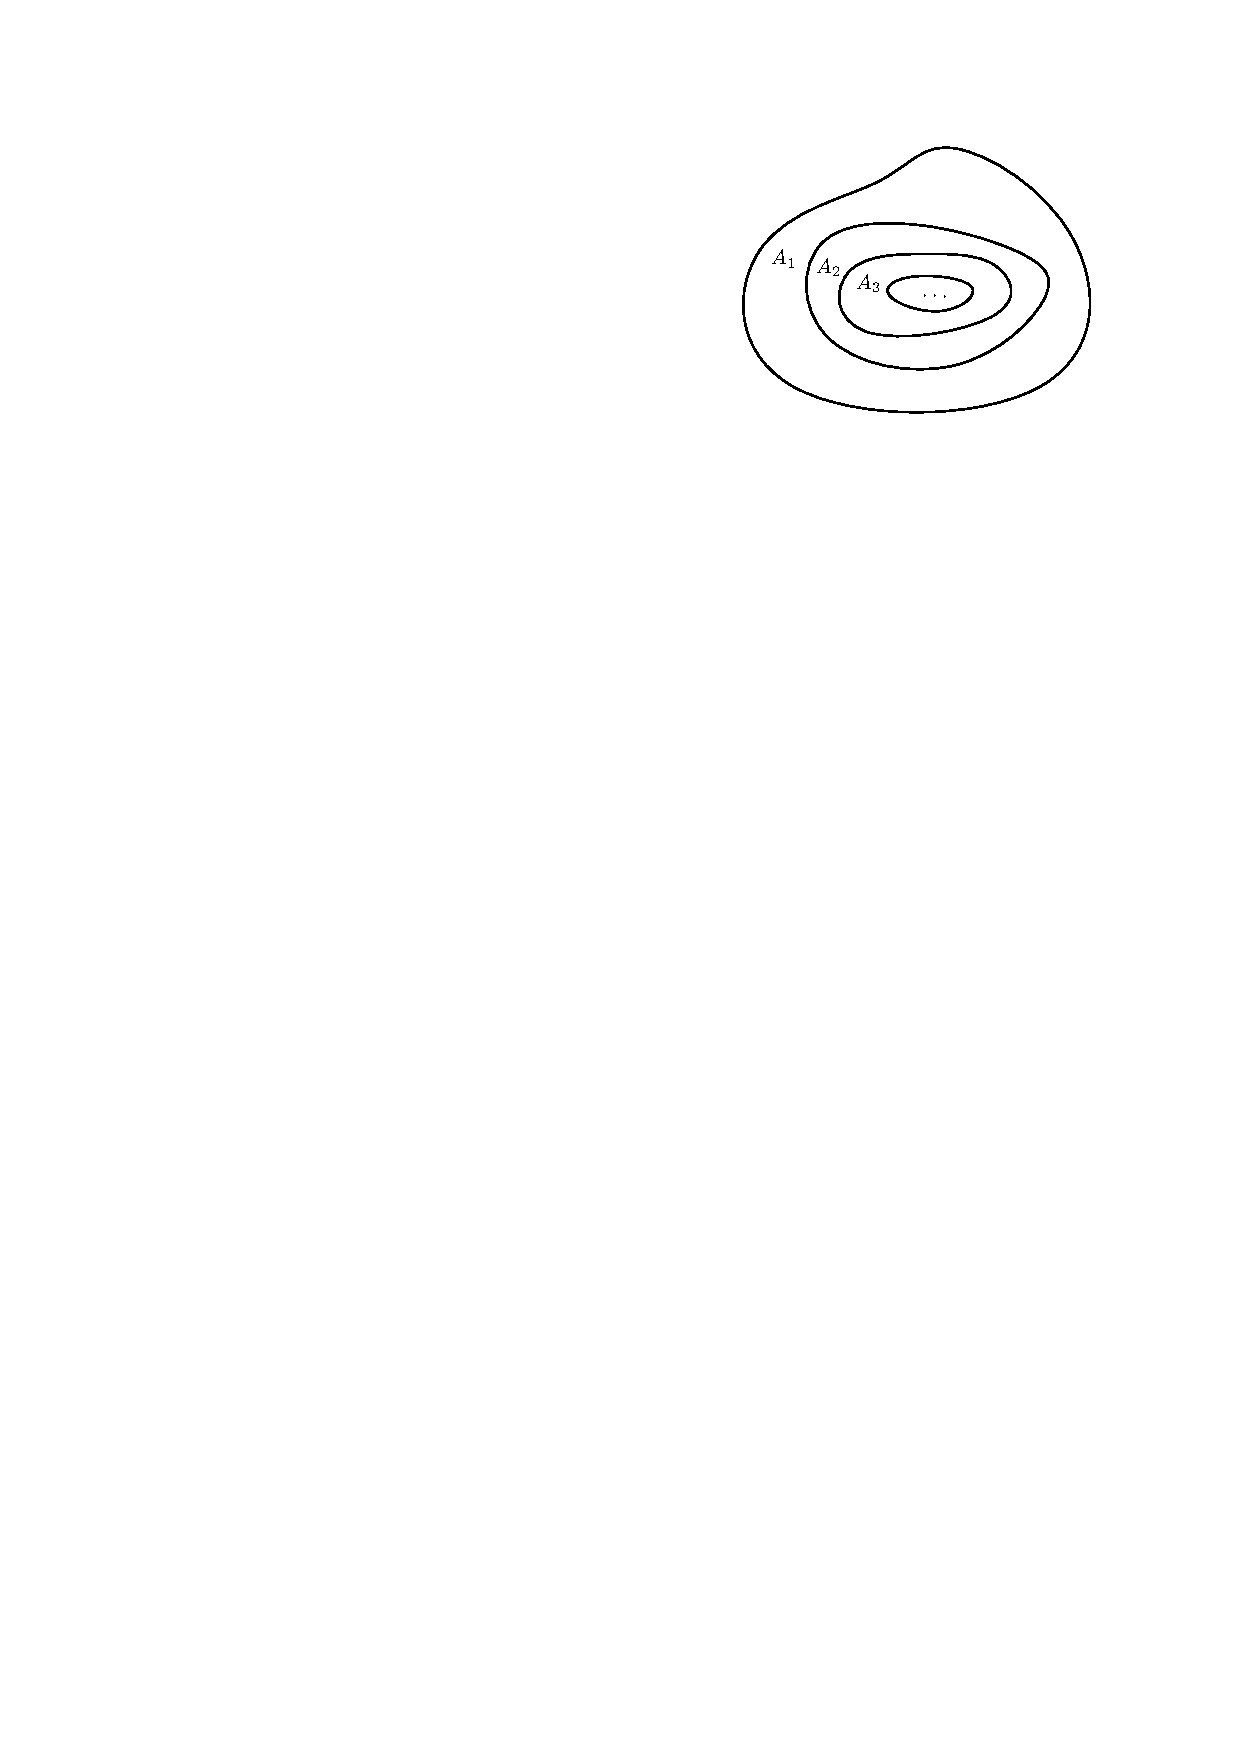
\includegraphics{ch02-nerostouci-posl-mnozin.pdf}
            \caption{Nerostoucí posloupnost množin}
            \label{fig:nerost-posl-mnozin}
        \end{subfigure}
        \caption{Ilustrace k~důkazu věty \ref{thm:mira-vlastnosti}}
    \end{figure}
    (Převzato z \citep[str. 19]{Netuka2016})
\end{proof}
\todo{Přidat obrázek ilustrující bod (v).}
\begin{remark}
    Předpoklad $\mu(A_1)<\infty$ ve větě \ref{thm:mira-vlastnosti} v~bodě \ref{thm:mira-nerost-posl} nelze vynechat. Jednoduchý protipříklad si uvedeme v~sekci \ref{sec:lebesgueova-mira}.
\end{remark}